\chapter{Preliminaries}\label{chap:models}
\markboth{Preliminaries}{}% To set left/right header
% \localtableofcontents

This chapter introduces the notion of \emph{closed-loop sensitivity}, which forms a key foundation of this thesis.
This concept quantifies how variations of some model parameters (supposed to be uncertain) affect the evolution of the system in closed-loop, i.e., by also taking into account any controller chosen for executing the task.
Then, it is presented how this sensitivity notion can be leveraged to derive \emph{uncertainty tubes} that bounds the system evolution both in the \emph{input} and \emph{state} spaces.
These tubes are subsequently used to enforce robust constraints within the several motion planning algorithms presented in this thesis.
Finally, the quadrotor and differential drive robot models used in this manuscript are introduced.

\section{Closed-loop sensitivity}\label{sec:sensi_and_tubes}

\subsection{Definition}\label{sec:sensi}

Consider an arbitrary dynamic system with a set of uncertain parameters $\p \in \mathbb{R}^{n_p}$ (i.e. parameters that are difficult to model).
The system dynamic can be described using the following set of \gls{odes}:
\begin{equation}\label{eq:dyna}
    \dot{\q}=\f(\q,\,\u,\,\p), \quad \q(t_0)=\q_{0},
\end{equation}
where $\q\in \mathbb{R}^{n_{q}}$ is the system state vector and $\u\in \mathbb{R}^{n_{u}}$ is the control input vector.
Also, assume the presence of a controller $\boldmu$ of any form whose aim is to track a \emph{desired trajectory} $\q_d(t)$ such that:
\begin{equation}\label{eq:ctrl}
     \left \{
     \begin{array}{l l}
          \dot{\bxi} = \g(\bxi,\,\q,\,\q_d,\,\p_n,\,\k_c,\,t), \quad \bxi(t_0)=\bxi_{0}, \\
          \u=\boldmu(\bxi,\,\q,\,\q_d,\,\p_n,\,\k_c,\,t), 
   \end{array} 
   \right .
\end{equation}
where $\bxi\in \mathbb{R}^{n_{\xi}}$ are the internal states of the controller (e.g., an integral action), $\k_{c}\in \mathbb{R}^{n_{k}}$ the controller gains, and $\p_{n}\in{\mathbb{R}^{n_{p}}}$ is the vector of "nominal" system parameters used in the control loop, i.e. the estimated nominal values of $\p$.

In line with the previous definitions, the following sections of this thesis will then differentiate between three types of state vectors of key importance:
\begin{enumerate}
  \item $\q_d$: The \emph{desired} system state vector which refers to the desired values of the controllable system states. This state vector is typically the output of a motion planner. Note that the dimension of this vector may differ from that of the real system because the vector represents a simplified or abstracted model, which might omit certain physical aspects or constraints that are present in the actual system, particularly in the case of under-actuated systems, where not all degrees of freedom are controlled.
  \item $\q_n$: The \emph{nominal} system state vector which represents the real state values of the system during the execution under nominal parameters (i.e. when the uncertain system parameters $\p$ perfectly match the parameter values used in the control loop $\p_n$). A distinction is made between the nominal states and the desired states, as they are generally not equal due to factors such as controller settings, transient behavior, etc.
  \item $\q$: The \emph{uncertain} system state vector which refers to the real state values of the system during the execution, influenced by a set of uncertain parameters.
\end{enumerate}
Note that the same notations apply to the control input vector as well (e.g., $\u_n$ represents the "nominal" control input values, i.e., when $\p=\p_n$).

It is possible to quantify how the presence of uncertain parameters (i.e. when the real system parameters $\p$ deviate from the nominal value $\p_n$ used in the control loop) affects the evolution of $\q(t)$ and $\u(t)$ according to the following matrices:
\begin{equation}\label{eq:sensi}
  \bPi(t)=\left.\frac{\partial \q(t)}{\partial \p}\right|_{\p=\p_n} \quad\quad \bTheta(t)=\left.\frac{\partial \u(t)}{\partial \p}\right|_{\p=\p_n}
\end{equation}
where $\bPi(t)\in \mathbb{R}^{n_q \times n_p}$ and $\bTheta(t)\in \mathbb{R}^{n_u \times n_p}$ are respectively defined in~\cite{cPi,cTh} as the \emph{state-sensitivity matrix} and the \emph{input-sensitivity matrix}.
A closed-form expression for Equation~(\ref{eq:sensi}) is, in general, not available. 
However, as shown in~\cite{cPi,cTh}, their evolution in time can be computed by differentiating Equation~(\ref{eq:sensi}) according to the following set of \myglsentry{odes}:
\begin{equation}\label{eq:dyna_sensi}
  \left \{
  \begin{array}{l l l}
       \dot{\bPi}(t) = \boldsymbol{\frac{\partial{f}}{\partial{q}}}\bPi+ \boldsymbol{\frac{\partial{f}}{\partial{u}}}\bTheta+ \boldsymbol{\frac{\partial{f}}{\partial{p}}}, \quad \bPi(t_0)=\bPi_0, \\
       \dot{\bPi}_{\xi}(t) = \boldsymbol{\frac{\partial{g}}{\partial{q}}}\bPi+ \boldsymbol{\frac{\partial{g}}{\partial{\xi}}}\bPi_{\xi}, \quad \bPi_{\xi}(t_0)=\bPi_{\xi0}, \\
       \bTheta(t) = \boldsymbol{\frac{\partial{h}}{\partial{q}}}\bPi+ \boldsymbol{\frac{\partial{h}}{\partial{\xi}}}\bPi_{\xi} 
  \end{array}
  \right .
\end{equation}
where $\bPixi(t)\in \mathbb{R}^{n_{\xi} \times n_p}$ represents the \emph{internal state sensitivity} matrix.

Now that the sensitivity matrices are defined, one can optimize the desired trajectory s.t. a norm of these matrices is minimized (see~\cite{cPi,cTh}). 
This optimization produces a trajectory s.t. the closed-loop evolution of $\q(t)$/$\u(t)$ closely matches its evolution in the nominal case $\q_n(t)$/$\u_n(t)$.

\subsection{Tube computation}\label{sec:tubes}

\begin{figure} [t]
  \centering
  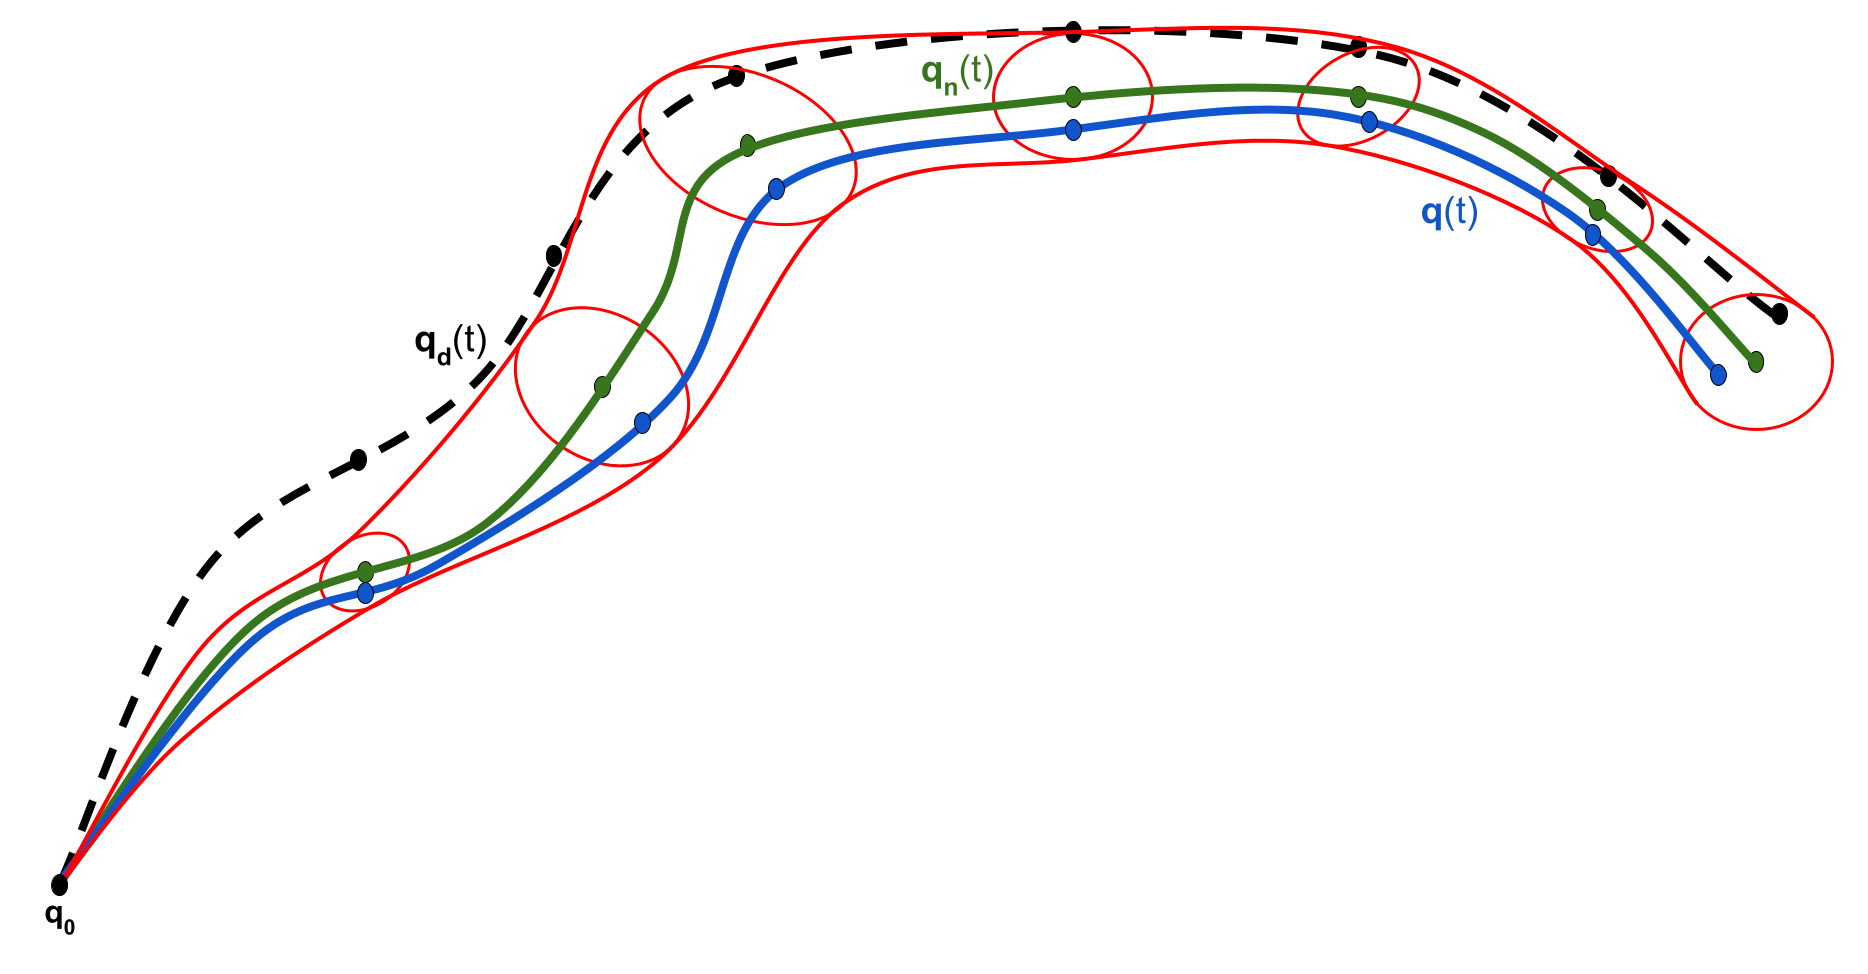
\includegraphics[width=0.8\linewidth]{figures/models/tubes.png} 
  \caption{Illustration of the uncertainty tube (red) and a perturbed trajectory $\q(t)$ (blue), centered around the nominal trajectory $\q_n(t)$ (green), which results from following the reference trajectory $\q_d(t)$ (dashed black).}%
  \label{fig:tubes}%
\end{figure}

\begin{figure} [t]
  \centering
  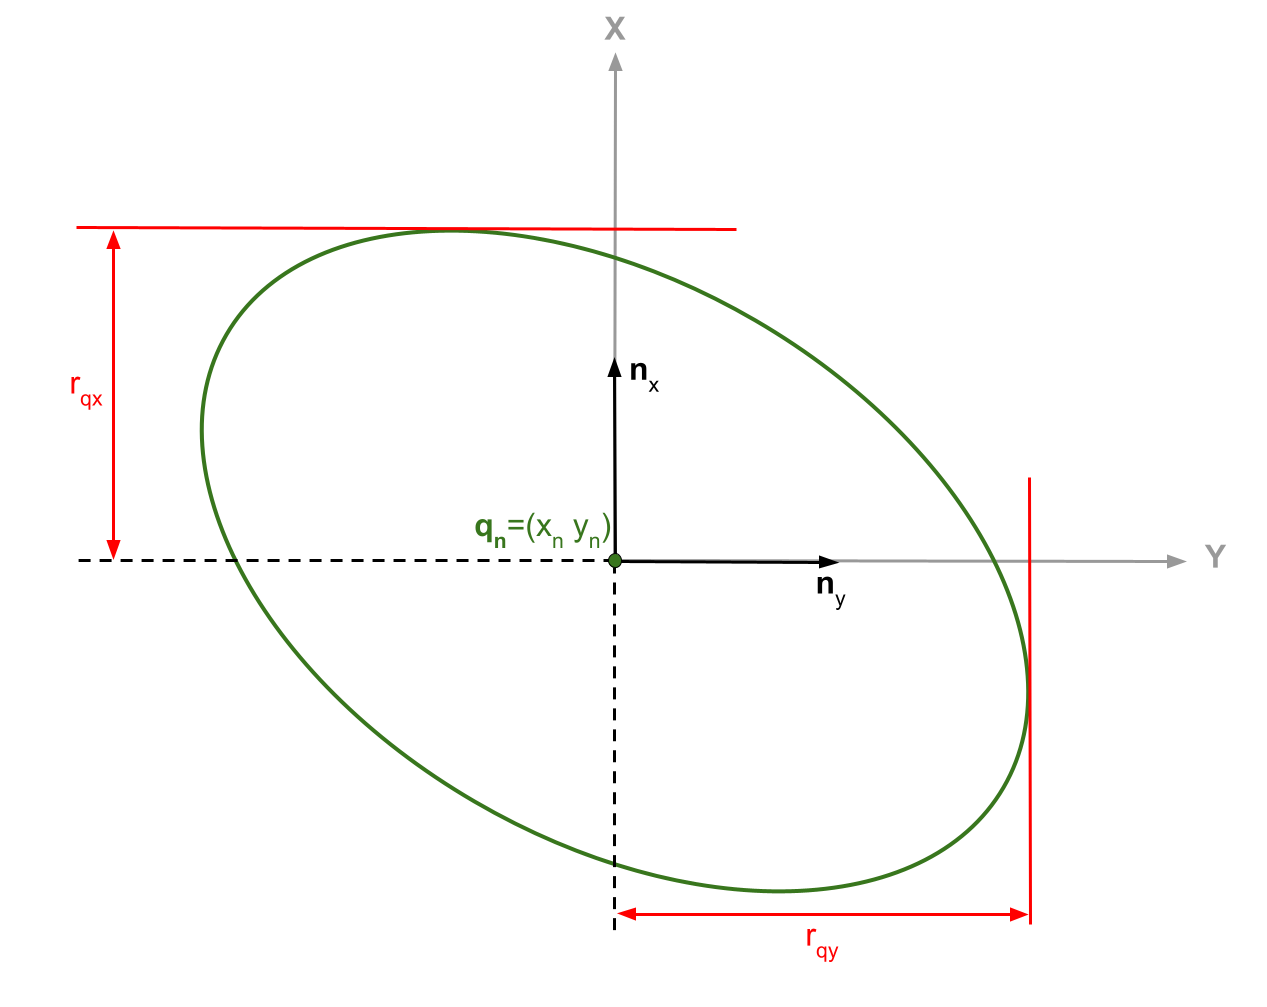
\includegraphics[width=0.6\linewidth]{figures/models/radius.png} 
  \caption{2D representation of an uncertainty ellipse (green) in the x-y state space centered at $\q_n$, along with the tube radius (red) that illustrates the worst-case deviations along each state space components.}%
  \label{fig:ellips_radius}%
\end{figure}

Another important feature of these matrices is their utility in deriving \emph{uncertainty tubes}, that bounds the closed-loop system trajectory $\q(t)$/$\u(t)$ around its nominal trajectory $\q_n(t)$/$\u_n(t)$ as shown in~\cite{cTube} and illustrated in Figure~\ref{fig:tubes}.
The following remind how to establish such bounds around the nominal state trajectory $\q_n(t)$ by focusing solely on the state-sensitivity matrix $\bPi(t)$ for clarity. 
However, it is important to note that this same procedure can also be applied to compute bounds around the nominal input trajectory $\u_n(t)$ by leveraging the input-sensitivity matrix $\bTheta(t)$.

The uncertainty tube for each component of the state is characterized by a \emph{radius} which bounds the state component evolution from its nominal value over time, i.e. for the $i$-th component of the state ($q_i(t)$) the tube radius $r_{q,i}(t)$ is defined s.t.:
\begin{equation}\label{eq:bounds_q}
  q_{n,i}(t) - r_{q,i}(t) \leq q_i(t) \leq q_{n,i}(t) + r_{q,i}(t).
\end{equation}

Let $\Delta\q(t) = \q(t) - \q_n(t)$, representing the deviation of the perturbed trajectory from the nominal one, which we seek to bound.
Assume that for each uncertain parameter $p_{i \in [1, n_p]}$ in $\p$, we have a bounded parameter deviation $\delta p_i \in \mathbb{R}$ s.t. 
\begin{equation*}
  \forall i \in [1, n_p] ,p_i \in [p_{n_i}-\delta p_i, p_{n_i}+\delta p_i].
\end{equation*}
Such deviations can be mapped into the parameter space by mean of the following ellipsoid
\begin{equation}\label{eq:p_ellipsoid}
  \Delta\p^T \bW^{-1} \Delta\p \leq 1,
\end{equation}
where $\bW$ is the following diagonal weight matrix
\begin{equation*}
  \bW = \begin{bmatrix}
    \delta p_1^2 & 0 & \cdots & 0 \\
    0 & \delta p_2^2 & \cdots & 0 \\
    \vdots & \vdots & \ddots & \vdots \\
    0 & 0 & \cdots & \delta p_{n_p}^2
    \end{bmatrix} \in \mathbb{R}^{n_p \times n_p}.
\end{equation*}

Assuming small parameters variations (i.e. small $\delta \p$) it is possible to perform a first-order approximation around the nominal trajectory $\q_n(t)$ to obtain 
\begin{equation}\label{eq:approx}
  \Delta\q(t) =  \q(t) - \q_n(t) \approx \bPi(t) \Delta\p.
\end{equation}

Without loss of generality, for a well-chosen $\delta \p$ s.t. Equation~(\ref{eq:approx}) holds, ~\cite{cTube} has shown how to map the parameters ellipsoid from Equation~(\ref{eq:p_ellipsoid}) in the system state space in order to obtain the corresponding uncertainty ellipsoid
\begin{equation}\label{eq:q_ellipsoid}
  \Delta\q(t)^T (\bPi(t) \bW \bPi(t)^T)^\dag \Delta\q(t) \leq 1.
\end{equation}
However, it is important to note that the ellipsoid axes are in general not aligned with the canonical basis of the state space.
This implies that computing the deviation of each state component $q_i(t)$ is not straightforward, as direct use of the ellipsoid semi-axes length is not possible and the direction of interest may not belong to the range of the ellipsoid.

Nevertheless, it has been shown in ~\cite{cTube} how to obtain the tube radius along the $i$-th component of the state $q_i(t)$ by mean of the following projection:
\begin{equation}\label{eq:radius}
  r_{q,i}(t) =  \sqrt{\boldsymbol{n_i}^{T} \boldsymbol{K_{\Pi}}(t) \boldsymbol{n_i}},
\end{equation}
where $\boldsymbol{n}_i$ is the unit-norm vector of the $i$-th state space component, and $\boldsymbol{K_{\Pi}}(t) = \boldsymbol{\Pi}(t)\boldsymbol{W}\boldsymbol{\Pi}(t)^T$ is the kernel matrix of Equation~(\ref{eq:q_ellipsoid}).
It is important to note that the radius along the $i$-th component represents the maximum possible deviation in that direction and does not directly correspond to the semi-axes of the uncertainty ellipsoid as depicted in Figure~\ref{fig:ellips_radius}.

Finally, it is important to remind that since the uncertainty tube radii depend on the state sensitivity $\boldsymbol{\Pi}(t)$, it is necessary to solve the set of \myglsentry{odes} represented by Equation~(\ref{eq:dyna}), Equation~(\ref{eq:ctrl}), and Equation~(\ref{eq:dyna_sensi}) beforehand.
Additionally, note how, in general, the tube radius does not necessarily increase monotonically due to the influence of feedback action as illustrated in Figure~\ref{fig:tubes}, despite the cumulative effect of uncertainties over time. 

\section{Models considered in this thesis}

To demonstrate the versatility of the approaches proposed in this thesis across various robots and controllers, a quadrotor and a differential drive robot are both considered in this manuscript, along with two distinct controllers and interpolation methods, which are detailed in the following sections.

\subsection{Quadrotor robot} \label{sec:quad_model}

\subsubsection{Dynamic model}

\begin{figure} [t]
    \centering
    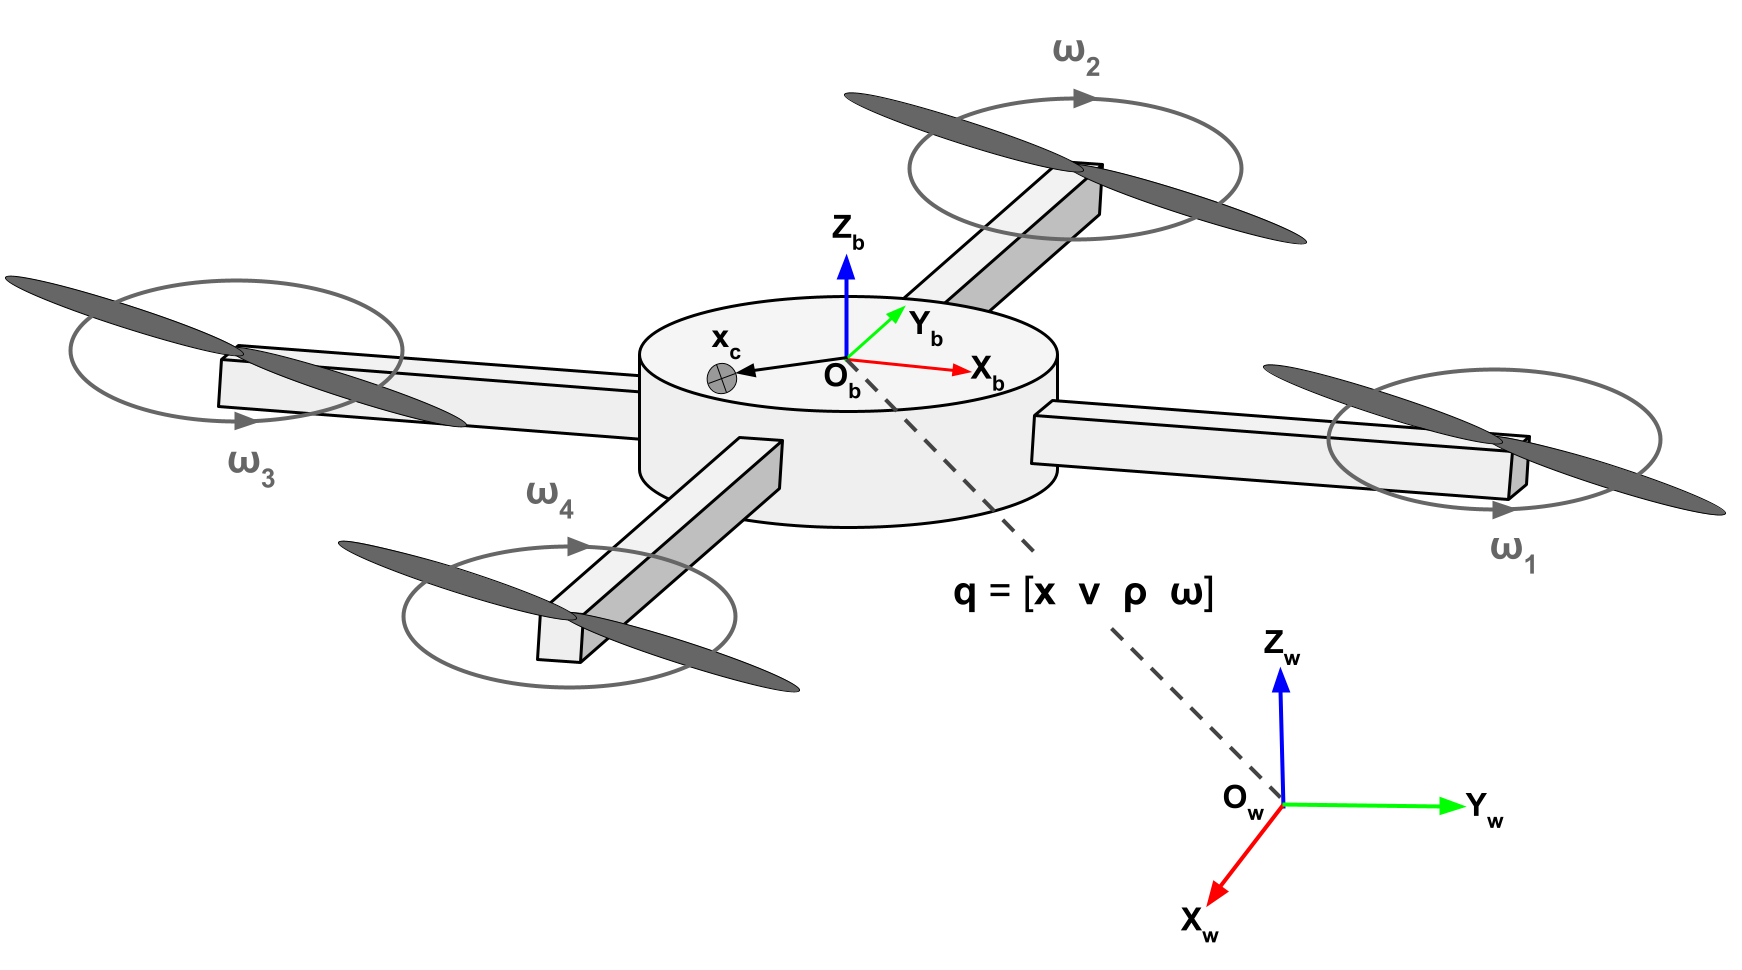
\includegraphics[width=0.8\linewidth]{figures/models/drone.png} 
    \caption{Quadrotor robot representation with a shift in the center of mass.}%
    \label{fig:quad}%
\end{figure}

Let the ENU (East North Up) world frame be defined as $F_W \allowbreak = \allowbreak \{O_W, \allowbreak X_W, \allowbreak Y_W, \allowbreak Z_W\}$ and $F_B = \allowbreak\{O_B, \allowbreak X_B, \allowbreak Y_B, \allowbreak Z_B\}$ be the quadrotor body frame attached to its geometric center ($O_B$).
The state of the quadrotor is defined as $\boldsymbol{q} = [\boldsymbol{x}  \, \boldsymbol{v} \, \boldsymbol{\rho} \, \boldsymbol{\omega}]$ where $\boldsymbol{x} = [x \, y \,z] \in \mathbb{R}^{3}$ and $\boldsymbol{v} = [v_x \, v_y \,v_z] \in \mathbb{R}^{3}$ are respectively the linear position and linear velocity vector of $O_B$ expressed in $F_W$. The body orientation w.r.t. $F_W$ is represented by the unitary quaternion $\boldsymbol{\rho}$ and its angular velocity as $\boldsymbol{\omega} = [\omega_x \, \omega_y \, \omega_z] \in \mathbb{R}^{3}$. 
Finally, let $\boldsymbol{R(\rho)}$ be the rotation matrix associated to $\boldsymbol{\rho}$.

Let the control input vector $\u = [\omega_{1}^2 \, \omega_{2}^2 \, \omega_{3}^2 \, \omega_{4}^2]^T$ represent the squared rotor speeds. 
The vector $\u$ is related to the total propeller thrust $f$ and torques $\boldsymbol{\tau}$ by mean of a standard allocation matrix $\boldsymbol{T}$ s.t.
\begin{equation}\label{eq:alloc_mat}
  \begin{bmatrix}
    f \\
    \boldsymbol{\tau}
    \end{bmatrix} = \boldsymbol{T}(l, k_f, k_{\tau}) \u,
\end{equation}
where $k_f$ and $k_{\tau}$ refer to the thrust and drag coefficients of the propellers respectively, and $l$ stands for the quadrotor arms length.
Also, consider that the \myglsentry{com} is displaced from the robot geometric center of an offset $\boldsymbol{x_{c}} = [x_{cx} \, x_{cy} \, x_{cz}]$ expressed in $F_B$ as depicted in Figure~\ref{fig:quad}. 
This displacement can occur due to onboard sensors, the presence of a payload, or other factors.
Under this consideration and according to Newton's second law, the total force ($\boldsymbol{f_{tot}}$) and torque ($\boldsymbol{\tau_{tot}}$) acting on the quadrotor can be expressed by taking an additional fictitious force due to the displaced \myglsentry{com} in $F_B$ s.t. 
\begin{equation}\label{eq:quad_newton}
    \begin{array}{@{}l@{}l@{}}
        \boldsymbol{f_{tot}} &= f Z_W - mg\boldsymbol{R(\rho)}^TZ_W-m[\boldsymbol{\omega}]_{\times}[\boldsymbol{\omega}]_{\times}\boldsymbol{x_c} 
          
          \\
      
       \boldsymbol{\tau_{tot}} &= \boldsymbol{\tau}-mg[\boldsymbol{x_c}]_{\times}\boldsymbol{R(\rho)}^{T}Z_W - [\boldsymbol{\omega}]_{\times}\boldsymbol{J}\boldsymbol{\omega}
  \end{array}
\end{equation}
where $m$ is the mass and $\boldsymbol{J}$ is the inertia matrix of the system. 

By considering the spatial inertia matrix
\[
\boldsymbol{S} =   \left( {\begin{array}{cc}
    m\boldsymbol{I_3} & -m[\boldsymbol{x_c}]_{\times} \\
    m[\boldsymbol{x_c}]_{\times} & \boldsymbol{J} \\
  \end{array} } \right)
\]
one finally gets the body frame linear acceleration $\boldsymbol{\alpha}$ and angular acceleration $\boldsymbol{\eta}$
as: 
$
\left( 
    \boldsymbol{\alpha}^T \; \boldsymbol{\eta}^T \right)^T 
  =
  \boldsymbol{S}^{-1}
  \left( \boldsymbol{f_{tot}}^T \;
    \boldsymbol{\tau_{tot}}^T \right)^T. 
$
The dynamic model is then defined as follows:
\begin{equation}\label{eq:quad_dynamic}
    \Dot{\q}
    =
     \left \{
     \begin{array}{l l}
           \dot{\boldsymbol{x}} = \boldsymbol{v} \\
           
           \dot{\boldsymbol{v}}= \boldsymbol{\alpha} \\

           \dot{\boldsymbol{\rho}}=\frac{1}{2}
               \boldsymbol{\rho} \otimes \begin{bmatrix}
                                          0 \\
                                          \boldsymbol{\omega}
                                          \end{bmatrix} \\
           
           \dot{\boldsymbol{\omega}}=\boldsymbol{\eta}
   \end{array}
   \right . 
\end{equation}
In line with Section~\ref{sec:sensi}, let the vector $\p = [m \, x_{cx} \, x_{cy} \, x_{cz} \, J_{x} \, J_{y} \,J_{z} \, k_f \, k_{\tau}]^T \in \mathbb{R}^{9}$ represent all the parameters used in the robot model outlined above that are subject to uncertainty. 
This vector can be adjusted based on the various scenarios presented in this thesis.

Finally, as tracking controller, we consider the widely used Lee (or geometric) controller~\cite{cLee} to computes the control input vector $\u$.
This controller takes advantage of the well-known quadrotor flat outputs ~\cite{cFlat} to track a desired trajectory defined as $\q_d(t) = [\boldsymbol{x}_d(t) \, \boldsymbol{v}_d(t) \, \boldsymbol{a}_d(t) \, \psi_d(t) \, \Dot{\psi}_d(t)]^T \in \mathbb{R}^{11}$ respectively composed of the desired linear positions, velocities, accelerations, yaw orientation angle, and yaw angular velocity.
Note that, since the quadrotor is an under-actuated system, not all states can be controlled. This is why only the desired yaw angle is incorporated into the desired trajectory.

Let the linear position error and linear velocity error be defined as follows:
\begin{equation}\label{eq:pos_error}
  \boldsymbol{e_x}(t) = \boldsymbol{x}(t) - \boldsymbol{x}_d(t) \in \mathbb{R}^3, \,
  \boldsymbol{e_v}(t) = \boldsymbol{v}(t) - \boldsymbol{v}_d(t) \in \mathbb{R}^3,
\end{equation}
and the controller gains vector \(\boldsymbol{k}_c = [\boldsymbol{k}_{x}^T \, \boldsymbol{k}_{v}^T \, \boldsymbol{k}_{R}^T \, \boldsymbol{k}_{\omega}^T]^T \in \mathbb{R}^{12}\) with their associated diagonal representation $(\boldsymbol{K_x}, \boldsymbol{K_v}, \boldsymbol{K_R}, \boldsymbol{K_\omega}) \in (\mathbb{R}^{3\times3})^4$.
This control strategy starts by computing the desired third basis vector of the body frame:
\begin{equation}
  \boldsymbol{r}_{3d} = \frac{-\boldsymbol{K_x} \cdot \boldsymbol{e_x} - \boldsymbol{K_v} \cdot \boldsymbol{e_v} + m(g Z_W + \boldsymbol{a}_d) }{\left\| -\boldsymbol{K_x} \cdot \boldsymbol{e_x} - \boldsymbol{K_v} \cdot \boldsymbol{e_v} + m(g Z_W + \boldsymbol{a}_d) \right\|} \in \mathbb{R}^3.
\end{equation}
Then, using the desired yaw angle $\psi_d$, the desired heading vector can be defined as $\boldsymbol{\Omega_{\psi_d}} = [cos(\psi_d) \, sin(\psi_d) \, 0]^T$.
This heading vector is then used to compute the desired first and second basis vectors of the body frame:
\begin{equation}
  \boldsymbol{r}_{2d} = \frac{\left[\boldsymbol{r}_{3d}\right]_{\times} \cdot \boldsymbol{\Omega}_{\psi_d}}{\left\|\left[\boldsymbol{r}_{3d}\right]_{\times} \cdot \boldsymbol{\Omega}_{\psi_d}\right\|} \in \mathbb{R}^3, \, \boldsymbol{r}_{1d} = \left[\boldsymbol{r}_{2d}\right]_{\times} \cdot \boldsymbol{r}_{3d} \in \mathbb{R}^3.
\end{equation}
From the three body frame basis vectors it is then possible to define the desired rotation matrix $\boldsymbol{R}_d(\psi_d, t) = [\boldsymbol{r}_{1d} \, \boldsymbol{r}_{2d} \, \boldsymbol{r}_{3d}]$, and to compute the following attitude error:
\begin{equation}\label{eq:att_error}
  \boldsymbol{e_R}(t) = \frac{1}{2}[\boldsymbol{R}_d(\psi_d, t)^T \cdot \boldsymbol{R}(\boldsymbol{\rho}, t) - \boldsymbol{R}(\boldsymbol{\rho}, t)^T \cdot \boldsymbol{R}_d(\psi_d, t)^T]^\vee \in \mathbb{R}^3.
\end{equation}
Finally, to simplify the overall controller design, the desired yaw rate $\Dot{\psi}_d$ is always set to zero in this thesis, allowing the angular velocity error to be expressed as:
\begin{equation}\label{eq:rate_error}
  \boldsymbol{e_\omega}(t) = \omega(t) \in \mathbb{R}^3.
\end{equation}

According to the aforementioned errors, this control strategy computes the desired propeller thrust $f_d(t)$ and desired propeller torques $\boldsymbol{\tau}_d(t)$ that allow the tracking of the desired trajectory $\q_d(t)$:
\begin{equation}\label{eq:desftau}
  \left \{
    \begin{array}{l l}
      f_d(t) &= \left( -\boldsymbol{K_x} \cdot \boldsymbol{e_x}(t) - \boldsymbol{K_v} \cdot \boldsymbol{e_v}(t) + m(g Z_W + \boldsymbol{a}_d(t)) \right)^T \cdot (\boldsymbol{R}(\boldsymbol{\rho}, t) \cdot Z_W) \\
      \boldsymbol{\tau}_d(t) &= -\boldsymbol{K_R} \cdot \boldsymbol{e_R}(t) - \boldsymbol{K_\omega} \cdot \boldsymbol{e_\omega}(t)
    \end{array}
  \right .
\end{equation}
Note that the choice of setting the desired yaw rate to zero cancels terms in the expression of $\boldsymbol{\tau}_d(t)$ compared to the original expression in ~\cite{cLee}.

Finally, the control input vector $\u$ can be computed using the same standard allocation matrix $\boldsymbol{T}$ from Equation~\ref{eq:alloc_mat} using nominal parameters denoted $\boldsymbol{T}_n$ s.t.:
\begin{equation}\label{eq:control_lee}
  \u = \boldsymbol{T}_n^{-1}\begin{bmatrix}
        f_d \\
        \boldsymbol{\tau}_d
      \end{bmatrix}.
\end{equation}
Note that under nominal case (i.e. when $\p = \p_n$), $\boldsymbol{T} = \boldsymbol{T}_n$; thus, the propeller thrust and torques applied to the real system, as for $f$ and $\boldsymbol{\tau}$ in Equation~\ref{eq:quad_newton}, perfectly match the desired thrust and torques computed by the control law.
Note also that no internal controller states are considered in this controller; therefore, Equation~\ref{eq:dyna_sensi} simplifies to:
\begin{equation}\label{eq:dyna_sensi_simp}
  \left \{
  \begin{array}{l l}
       \dot{\bPi}(t) = \boldsymbol{\frac{\partial{f}}{\partial{q}}}\bPi+ \boldsymbol{\frac{\partial{f}}{\partial{u}}}\bTheta+ \boldsymbol{\frac{\partial{f}}{\partial{p}}}, \quad \bPi(t_0)=\bPi_0, \\\\
       \bTheta(t) = \boldsymbol{\frac{\partial{\eta}}{\partial{q}}}\bPi 
\end{array}
\right .
\end{equation}

\subsubsection{State interpolation}\label{sec:kinosplines}

With the quadrotor model and controller now defined, this section presents the interpolation method (hereafter referred to as the \emph{local} planner) for computing a desired trajectory that the geometric controller will track.

Given an initial desired state $\q_d^0 = [\boldsymbol{\gamma}^0 \, \boldsymbol{\Dot{\gamma}}^0 \, \boldsymbol{\Ddot{\gamma}}^0] \in \mathbb{R}^{12}$ and a goal state $\q_d^F = [\boldsymbol{\gamma}^F \, \boldsymbol{\Dot{\gamma}}^F \, \boldsymbol{\Ddot{\gamma}}^F] \in \mathbb{R}^{12}$ for the quadrotor, where $\boldsymbol{\gamma} = [x_{d} \, y_{d} \, z_{d} \, \Psi_{d}]^T \in \mathbb{R}^{4}$ represents the desired position along the x, y, and z axes and the desired yaw angle, the \emph{kino-spline} method from~\cite{cKino} is employed to plan a time optimal and continuous desired trajectory $\q_d(t)$ connecting $\q_d^0$ and $\q_d^F$. 

The trajectory generation problem is solved independently for each component of $\boldsymbol{\gamma}$.
Furthermore, in order to generate smooth trajectories in a global context, the local planner ensures the continuity of their derivatives up to the jerk (acceleration derivative). 
Note that even if the yaw angular acceleration is not required by the control law of Section~\ref{sec:quad_model}, the initial and goal yaw angular accelerations are used to ensure the smoothness of the generated trajectory. 
As for both initial and goal jerk, they are set to zero to facilitate a smooth transition between trajectories, and are therefore not considered in $\boldsymbol{\gamma}$.
Finally, the kino-spline method also consider bounds on the several derivatives up to the snap (i.e. $v_{max}, a_{max}$, etc.) and plan the trajectory accordingly.

As previously mentioned, this local planner focuses on generating local trajectories that are time optimal, i.e. that minimize the total time needed to reach $\q_d^F$.
This is achieved by reaching the full speed as soon as possible and by maintaining it as long as possible for each component of $\boldsymbol{\gamma}$.
This also implies that the time spent reaching this velocity must be minimized, which means that the time spent at maximum acceleration during transient phases must be maximized.
The same principle applies to jerk and snap; during variations in acceleration, the maximum achievable jerk should be maintained for as long as possible, while the duration of jerk variation phases is minimized.
This is achieved through a straightforward bang-bang snap method, which aims to maximize the time spent at maximum snap during the jerk transient phases.
By doing so, the duration of transient phases is minimized, and gradually, the duration of the maximum speed phase is maximized.
The principle of this trajectory generation is illustrated by Figure~\ref{fig:kino}.

\begin{figure} [t]
  \centering
  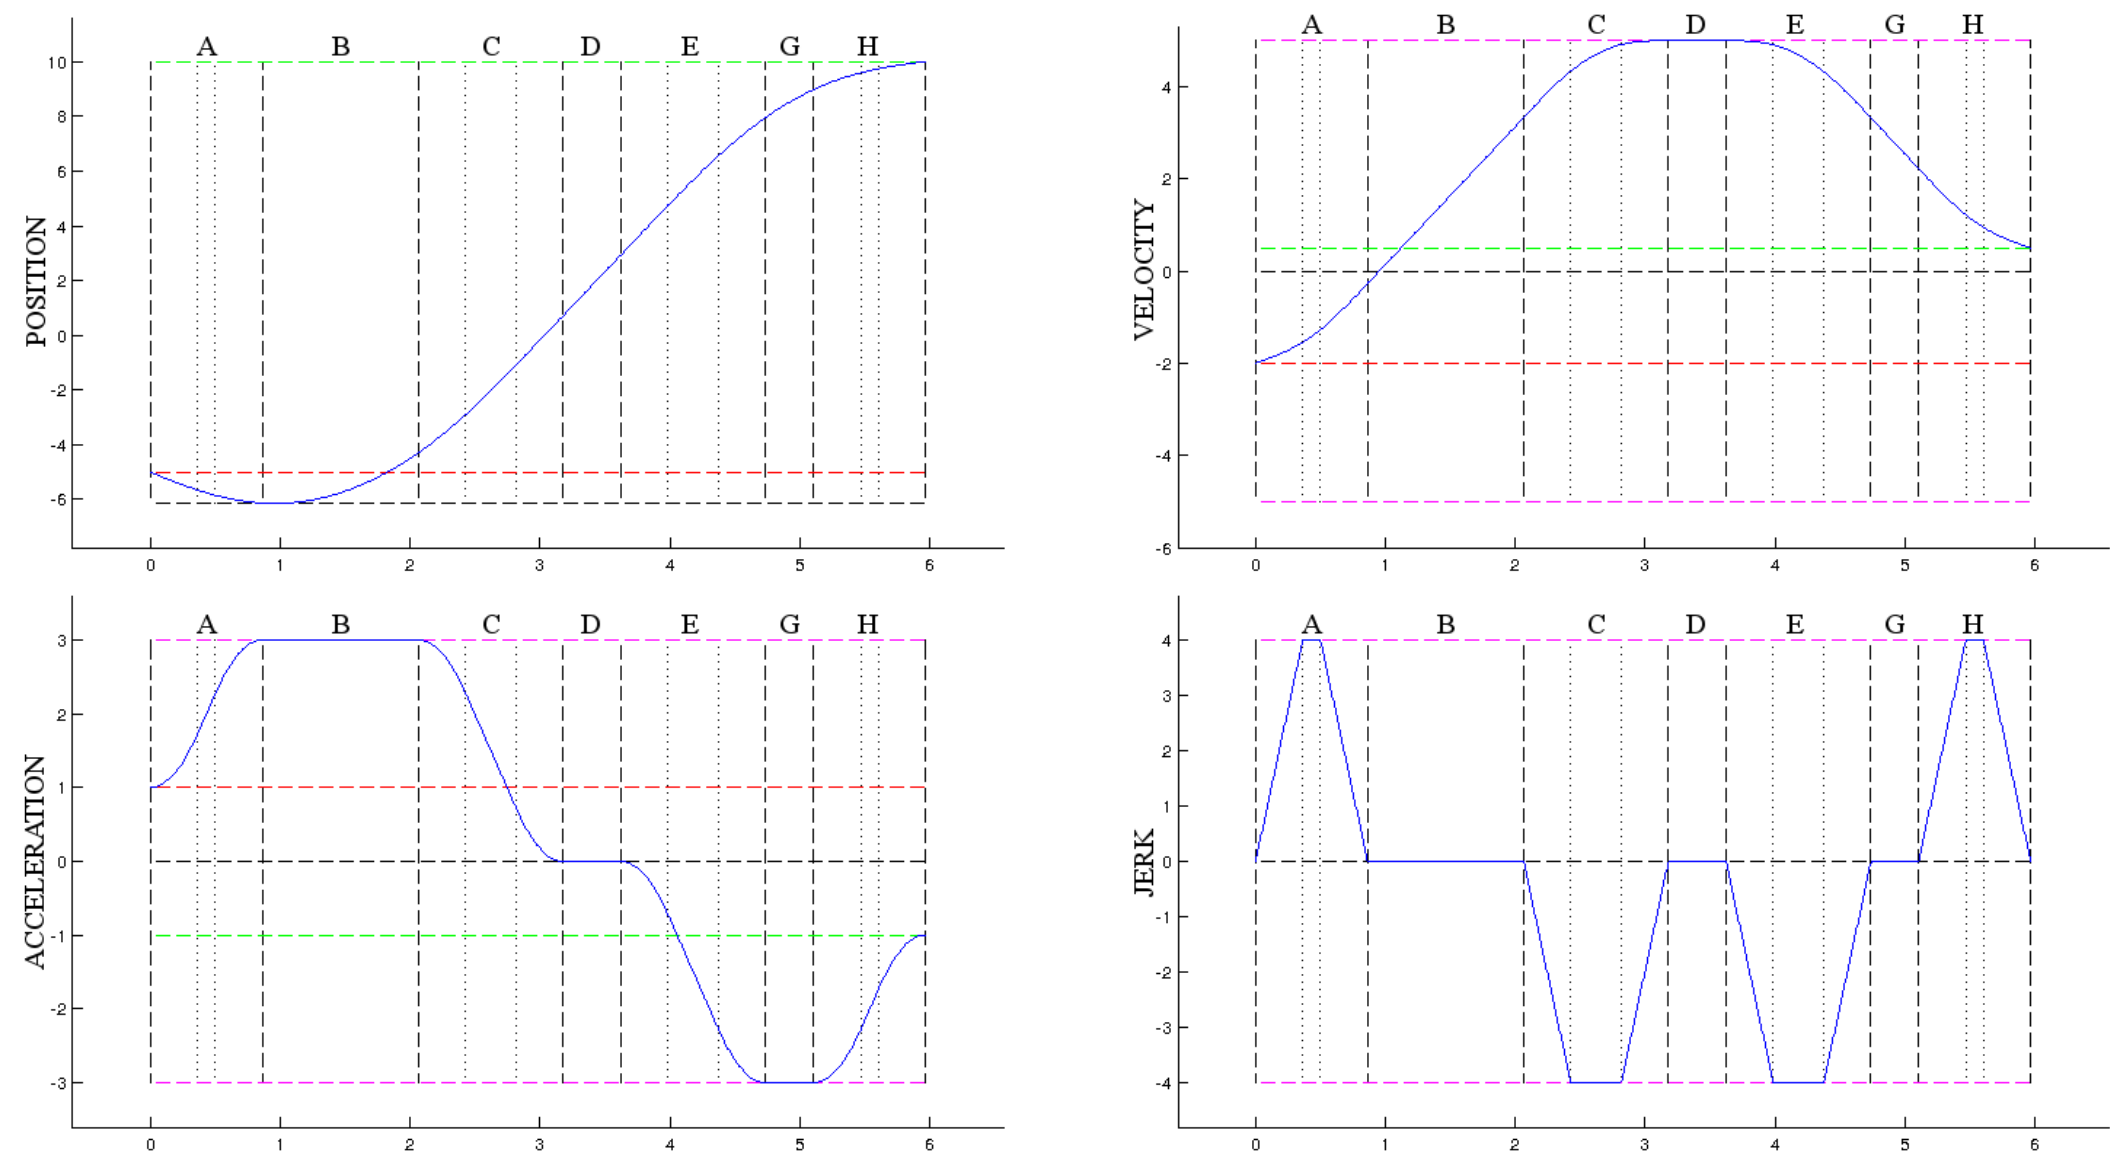
\includegraphics[width=0.99\linewidth]{figures/models/kino.png} 
  \caption{Example of a trajectory generated by the local planner for a single coordinate. The pink dashed lines indicate the bounds for each derivative, while the red and green dashed lines represent the initial and final values, respectively. 
  The letters A, B, C, D, E, G, and H represent the different phases that need to be minimized or maximized during the trajectory planning process.(extracted from~\cite{cKino})}%
  \label{fig:kino}%
\end{figure}

\subsection{Differential drive robot}\label{sec:unic_model}

\subsubsection{Dynamic model}

\begin{figure} [t]
  \centering
  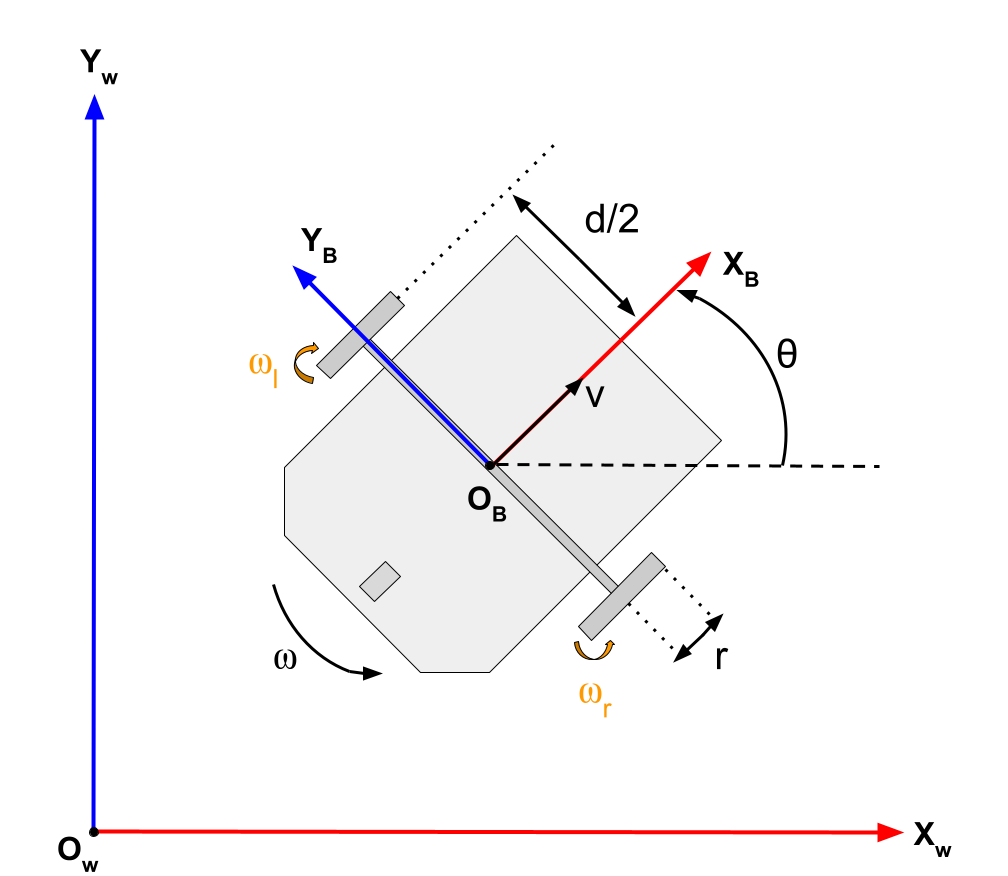
\includegraphics[width=0.6\linewidth]{figures/models/unicycle.png} 
  \caption{Illustration of the main quantities characterizing the differential drive robot.}%
  \label{fig:unicycle}%
\end{figure}

Let the world frame be defined as $F_W \allowbreak = \allowbreak \{O_W, \allowbreak X_W, \allowbreak Y_W\}$ and $F_B = \allowbreak\{O_B, \allowbreak X_B, \allowbreak Y_B\}$ be the differential drive robot body frame attached to its geometric center ($O_B$).
The robot state is defined as $\boldsymbol{q} = [\boldsymbol{x} \, \theta] \in \mathbb{R}^3$ where $\boldsymbol{x} = [x, \, y] \in \mathbb{R}^2$ are the linear positions of $O_B$ in $F_W$ and $\theta$ is the body heading (see Figure~\ref{fig:unicycle}).

Define the control input vector $\u = [\omega_r \, \omega_l]^T \in \mathbb{R}^2$, where $(\omega_r, \, \omega_l)$ are respectively the right and left wheel angular velocity.
Let also the robot linear and angular velocities be denoted by $v$ and $\omega$, respectively.
The aforementioned linear and angular velocities are related to the control input vector by mean of an allocation matrix $\boldsymbol{T}$ s.t.:
\begin{equation}\label{eq:unic_alloc}
  \begin{bmatrix}
    v \\
    \omega
  \end{bmatrix}
  =
  \begin{bmatrix}
    \frac{r}{2} & \frac{r}{2}\\
    \frac{r}{2d} & \frac{-r}{2d}
  \end{bmatrix}
  \begin{bmatrix}
    \omega_r \\
    \omega_l
  \end{bmatrix}
  =
  \boldsymbol{T} \u,
\end{equation}
where $d$ stands for the length between the two wheels, and $r$ for wheel radius.

The differential drive robot dynamic is then expressed as:
\begin{equation}\label{eq:unic_dyna}
  \Dot{\q} = 
  \begin{bmatrix}
    cos(\theta) & 0 \\
    sin(\theta) & 0 \\
    0 & 1
  \end{bmatrix} \boldsymbol{T} \u.
\end{equation}
In line with Section~\ref{sec:sensi}, the vector of parameters used in the robot model outlined above that are subject to uncertainty is defined as $\p = [r \, d]^T \in \mathbb{R}^{2}$.

The control task is to let the robot positions $\boldsymbol{x}$ track desired positions $\boldsymbol{x}_d = [x_d, \, y_d] \in \mathbb{R}^2$.
The differential drive robot is an under-actuated system, which is why the heading is excluded from the tracking process; it is induced by the robot dynamic instead.

To perform the tracking task, a \myglsentry{dfl} controller is used (e.g. see~\cite{cDFL}).
This control strategy considers an extended desired trajectory $\q_d(t) = [\boldsymbol{x}_d(t) \, \dot{\boldsymbol{x}}_d(t) \, \ddot{\boldsymbol{x}}_d(t)]^T \in \mathbb{R}^6$, where $\Dot{\boldsymbol{x}}_d(t) \in \mathbb{R}^2$ denote the desired linear velocities, and $\ddot{\boldsymbol{x}}_d(t) \in \mathbb{R}^2$ are the desired linear accelerations.
This trajectory is tracked by mean of the following controller internal states $\boldsymbol{\xi} = [\xi_v \, \xi_x \, \xi_y]^T \in \mathbb{R}^3$, where $\xi_v$ stands for the dynamic extension of the differential drive robot linear velocity $v$ (see Figure~\ref{fig:unicycle}), and $(\xi_x, \, \xi_y)$ are integral actions. 

By differentiating the robot positions twice, one obtains the following equations for the robot linear accelerations:
\begin{equation*}
  \ddot{\boldsymbol{x}}
  = 
  \begin{bmatrix}
    cos(\theta) & -\xi_v sin(\theta) \\
    sin(\theta) & \xi_v cos(\theta) 
  \end{bmatrix} 
  \begin{bmatrix}
    \dot{v} \\
    \omega
  \end{bmatrix}
  = \boldsymbol{A} \begin{bmatrix}
    \dot{v} \\
    \omega
  \end{bmatrix}
\end{equation*}
This differentiation is essential for formulating the kinematic relationships that enable efficient tracking of the desired positions.

Let the following vectors:
\begin{equation}\label{eq:unic_control_law}
  \left \{
  \begin{array}{l l l}
       \dot{\boldsymbol{x}}_{\xi} = [cos(\theta)\xi_v \, sin(\theta)\xi_v]^T \\
       \boldsymbol{\xi}_{xy} = [\xi_x \, \xi_y]^T \\
       \boldsymbol{\varrho} = \boldsymbol{\ddot{x}}_d + k_v(\boldsymbol{\dot{x}}_d - \dot{\boldsymbol{x}}_{\xi}) + k_p(\boldsymbol{x}_{d} - \boldsymbol{x}) + k_i\boldsymbol{\xi}_{xy}
  \end{array}
  \right .
\end{equation}
where $k_v$, $k_p$ and $k_i$ are the controller gains, s.t. in the following chapters of this thesis, the controller gain vector is defined as $\boldsymbol{k}_c = [k_p, \, k_v \, k_i]^T \in \mathbb{R}^3$.

Without loss of generality, the dynamics of the internal control states can be expressed (refer to~\cite{cDFL} for further details) as follows:
\begin{equation}
  \dot{\boldsymbol{\xi}} = 
  \begin{bmatrix}
    \begin{bmatrix}1 & 0\end{bmatrix}\boldsymbol{A}^{-1}\boldsymbol{\varrho} \\
    \boldsymbol{x}_d - \boldsymbol{x}
  \end{bmatrix}, 
\end{equation}
and the control inputs as:
\begin{equation}
  \u = \boldsymbol{T}_n^{-1} 
  \begin{bmatrix}
    \xi_v \\
    \begin{bmatrix}0 & 1\end{bmatrix}\boldsymbol{A}^{-1}\boldsymbol{\varrho}
  \end{bmatrix},
\end{equation}
where $\boldsymbol{T}_n$ represent the same allocation matrix as in Equation~\ref{eq:unic_dyna} but evaluated on the nominal parameters $\p_n$.

\subsubsection{State interpolation}\label{sec:dubins}

Now that the dynamic of the differential drive robot and its controller are defined, this section presents the local planner used to generate the desired trajectory $\q_d(t) = [\boldsymbol{x}_d(t) \, \dot{\boldsymbol{x}}_d(t) \, \ddot{\boldsymbol{x}}_d(t)]^T \in \mathbb{R}^6$ that is tracked by the \myglsentry{dfl} controller.
The trajectory generation problem is addressed using Dubins curves~\cite{cDubins}, which are differentiated twice. 

This approach ensures smooth and continuous trajectories between two position $(x^0, y^0)$ and $(x^F, y^F)$ in the x-y plane for systems with constraints on turning radius and forward motion such as the differential drive robot.
The method takes advantage of specified initial and final tangents to the curve (e.g. the differential drive robot heading angle $\theta$, in this case) to create smooth curves that respect the turning constraints.
A Dubins curve is composed of three possible segment types: left turn, right turn, and straight line as depicted in Figure~\ref{fig:dubins}. 
Each segment is designed with an optimal distance, arranged to create the shortest path between the two points $(x^0, y^0)$ and $(x^F, y^F)$. 
This configuration results in one of six possible combinations of segments (e.g., left-straight-right), producing a smooth, continuous path that meets the system turning and heading requirements.

In this thesis, the robot state used to compute such path is defined as $\boldsymbol{\gamma} = [x \, y \, \theta] \in \mathbb{R}^3$.
Once the path is computed, the x and y components are discretized using a given time step and then differentiated to obtain the corresponding desired velocities and accelerations required by Equation~\ref{eq:unic_control_law}.
Note that, although the heading is not directly controlled, a desired heading is specified to satisfy the tangent constraints.

\begin{figure} [t]
  \centering
  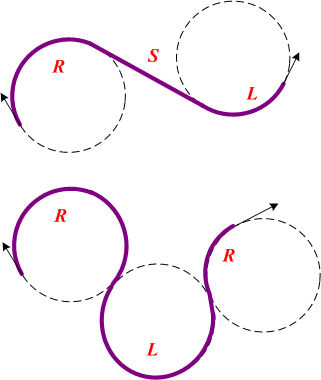
\includegraphics[width=0.4\linewidth]{figures/models/dubins.png} 
  \caption{Illustration of two possible Dubins paths: (top) a right turn, followed by a straight segment, then a left turn; (bottom) a right turn, followed by a left turn, then another right turn. (extracted from~\cite{cFigDubins})}%
  \label{fig:dubins}%
\end{figure}